\section{滤波}
相关命令:\nameref{cmd:bandpass}、\nameref{cmd:lowpass}、
\nameref{cmd:highpass}、\nameref{cmd:bandrej}

几乎所有的数据分析都需要将数据限制在一定的频率范围内,这就需要对数据做
各种不同方式的滤波。关于滤波的细节,可以参考滤波命令的相关说明,以及
信号处理相关书籍。至于滤波的范围,则依赖于具体的研究对象。

滤波过程中,有几个可以调节的参数:截止频率、阶数、通道数等等。不同的
参数对波形造成的变形有多大区别?不同的参数得到的滤波器的频率响应又是
怎样的?其实很容易就可以知道。

下面的代码生成了一个脉冲函数,然后对脉冲函数用某个参数组合做滤波,得到
滤波后的波形,然后对波形做FFT,得到波形的振幅谱和相位谱。根据定义可知,
得到的波形为滤波器的时间响应,得到的振幅谱和相位谱为滤波的频率响应:
\begin{SACCode}
SAC> fg impulse delta 0.01 npts 1000   // 生成脉冲函数, delta和npts可调
SAC> bp c 0.2 2 n 2 p 1                // 要查看的滤波参数
SAC> beginframe
SAC> xvport 0.1 0.9; yvport 0.7 0.9
SAC> fileid off
SAC> qdp off
SAC> title 'Time Domain Response'
SAC> p                                // 绘制时间域响应
SAC> fft
SAC> xvport .1 .45; yvport .15 .55
SAC> title 'Amplitude Response'
SAC> psp am loglog                    // 振幅响应
SAC> xvport .55 .9
SAC> title 'Phase Response'
SAC> psp ph linlin                    // 相位响应
SAC> endframe
\end{SACCode}
上面的代码涉及到了一些尚未介绍的命令,在后面会具体介绍。生成的效果图如下:
\begin{figure}[H]
\centering
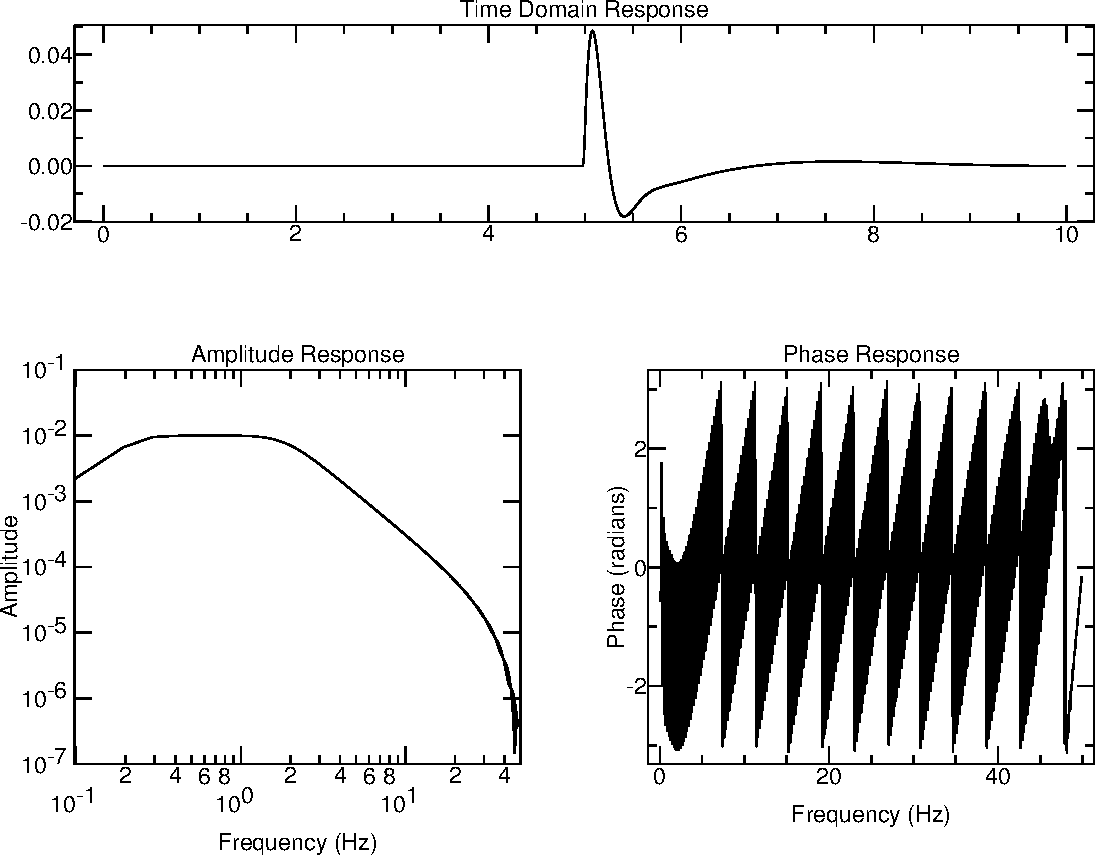
\includegraphics[width=0.8\textwidth]{filter-response}
\caption{滤波器的时间响应和频率响应}
\label{fig:filter-response}
\end{figure}

对脉冲波形做 \SI{0.5}{\Hz} 到 \SI{5}{\Hz} 的带通滤波,下图中给出了不同的
阶数和通道数对波形的影响:

\begin{figure}[H]
\centering
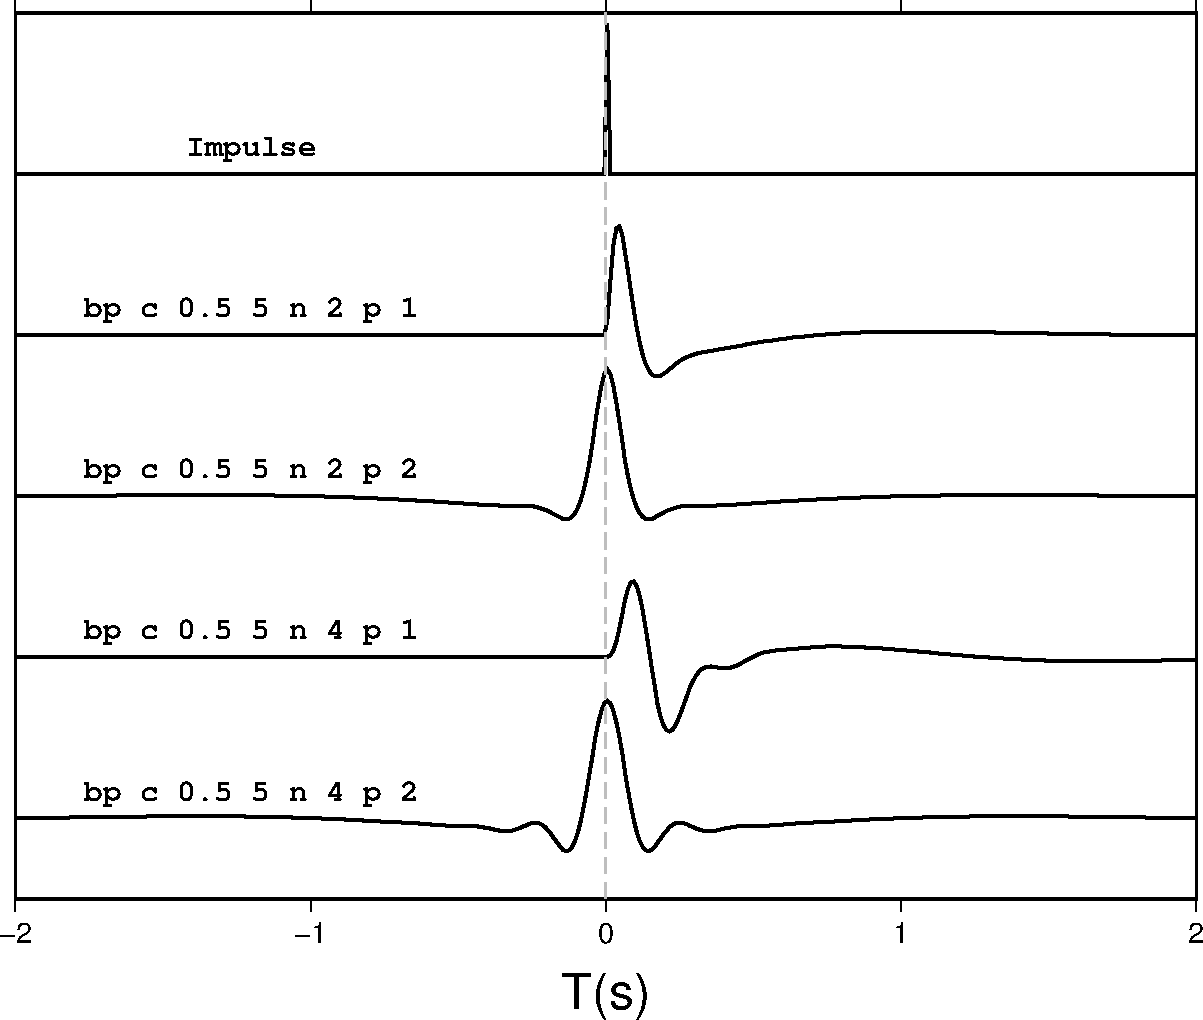
\includegraphics[width=0.8\textwidth]{filter-waveform}
\caption{不同参数的带通滤波效果}
\label{fig:filter-waveform}
\end{figure}
图 \ref{fig:filter-waveform} 中Impulse为原始脉冲波形,下面四条波形是分别
取不同的n值和p值的结果。

p取1时,对波形做一次带通滤波,由于滤波器存在相位延迟,因而导致波形的峰值
出现了时间延迟,因而会影响到震相的最大峰值的拾取,但对震相的初至却没有影响。

p取2时,对波形做正反两次带通滤波,此时不存在相位延迟,因而不会影响到最大
峰值的拾取,但震相的初至则存在时间上的提前。
